% ══════════════════════════════════════════════════════════════════════════════
% Response to midterm review comments (English) — companion to report.tex
% Build: LuaLaTeX, see .latexmkrc
% ══════════════════════════════════════════════════════════════════════════════
\documentclass[12pt]{article}

% ── Packages ──────────────────────────────────────────────────────────────────
\usepackage[margin=1in]{geometry}
\usepackage{amsmath, amssymb}
\usepackage{graphicx}
\usepackage{booktabs}
\usepackage[hidelinks]{hyperref}
\usepackage{caption}
\usepackage{float}

% ── Comment / response blocks ─────────────────────────────────────────────────
% \comment{<title>}{<reviewer text>} prints one numbered reviewer comment;
% the response follows as normal body text under \response.
\newcounter{comment}
\newcommand{\comment}[2]{%
  \refstepcounter{comment}%
  \par\bigskip\noindent\textbf{\thecomment.\ #1}\par\smallskip
  \noindent #2\par\medskip
}
\newcommand{\response}{\par\noindent\textbf{Response:}\par}

\title{Modeling and Evaluation of Spaceborne SAR Onboard Ship Detection\\
       Response to Midterm Review Comments}
\author{Jen-Tse Chen}
\date{October, 2026}

\pagestyle{plain}

\begin{document}

\maketitle

% ── Comment 1 ─────────────────────────────────────────────────────────────────
\comment{Equivalence of Eq.~(1) and Eq.~(6)}{%
  The data fidelity term in Eq.~(1) is
  defined in the raw echo domain ($\|Y - A(H)\|^2$), whereas the one in
  Eq.~(6) is defined in the image domain ($\|H - H_{\mathrm{CSA}}\|^2$).
  What is the theoretical basis for treating the two as equivalent?}

\response
The data fidelity terms in Eq.~(1) and Eq.~(6) are equal under the forward
operator used in this study, as shown below.

Following Bi \textit{et al.}~[6] in the report, $\mathcal{A}$ is taken as the
inverse of the CSA imaging operator $\mathcal{I}$, i.e., $\mathcal{A} =
\mathcal{I}^{-1}$. Let $\mathbf{y} = \mathrm{vec}(\mathbf{Y})$ and $\mathbf{h}
= \mathrm{vec}(\mathbf{H})$ be the vectorized echo and image. Since CSA is
linear, it can be written as a matrix $\boldsymbol{\Phi}$, so that
\begin{equation*}
  \mathbf{h}_{\mathrm{CSA}} = \boldsymbol{\Phi}\mathbf{y}, \qquad
  \mathrm{vec}\left(\mathcal{A}(\mathbf{H})\right)
    = \boldsymbol{\Phi}^{-1}\mathbf{h}.
\end{equation*}
The key property is that $\boldsymbol{\Phi}$ is unitary, i.e.,
$\boldsymbol{\Phi}^{H}\boldsymbol{\Phi} = \boldsymbol{\Phi}\boldsymbol{\Phi}^{H}
= \mathbf{I}$, and hence $\boldsymbol{\Phi}^{-1} = \boldsymbol{\Phi}^{H}$. Please
refer to Appendix~A for details of the vectorization, the matrix form of
$\boldsymbol{\Phi}$, and the proof of its unitarity. With this property,
the data fidelity term of Eq.~(1) becomes
\begin{align*}
  \left\|\mathbf{Y} - \mathcal{A}(\mathbf{H})\right\|_F^2
    &= \left\|\mathbf{y} - \boldsymbol{\Phi}^{-1}\mathbf{h}\right\|_2^2
    && \text{(vectorization preserves the norm)} \\
    &= \left\|\boldsymbol{\Phi}^{-1}\left(\mathbf{h}_{\mathrm{CSA}}
         - \mathbf{h}\right)\right\|_2^2
    && \text{(}\mathbf{y} = \boldsymbol{\Phi}^{-1}\mathbf{h}_{\mathrm{CSA}}\text{)} \\
    &= \left\|\boldsymbol{\Phi}^{H}\left(\mathbf{h}_{\mathrm{CSA}}
         - \mathbf{h}\right)\right\|_2^2
    && \text{(}\boldsymbol{\Phi}^{-1} = \boldsymbol{\Phi}^{H}\text{)} \\
    &= \left(\mathbf{h}_{\mathrm{CSA}} - \mathbf{h}\right)^{H}
       \boldsymbol{\Phi}\boldsymbol{\Phi}^{H}
       \left(\mathbf{h}_{\mathrm{CSA}} - \mathbf{h}\right)
    && \text{(}\|\mathbf{v}\|_2^2 = \mathbf{v}^{H}\mathbf{v}\text{)} \\
    &= \left(\mathbf{h}_{\mathrm{CSA}} - \mathbf{h}\right)^{H}
       \left(\mathbf{h}_{\mathrm{CSA}} - \mathbf{h}\right)
    && \text{(}\boldsymbol{\Phi}\boldsymbol{\Phi}^{H} = \mathbf{I}\text{)} \\
    &= \left\|\mathbf{h}_{\mathrm{CSA}} - \mathbf{h}\right\|_2^2
     = \left\|\mathbf{H}_{\mathrm{CSA}} - \mathbf{H}\right\|_F^2 .
\end{align*}
The two data fidelity terms are therefore equal, so Eq.~(1) with
$R(\mathbf{H}) = \|\mathbf{H}\|_1$ and Eq.~(6) are the same problem. In the
image-domain form of Eq.~(6), the problem decouples into independent
per-pixel problems, which gives the element-wise closed-form solution in
Eq.~(7). Invertibility alone is not sufficient: if $\boldsymbol{\Phi}$ were not
unitary, the fidelity term would become the weighted norm
$\|\boldsymbol{\Phi}^{-1}(\mathbf{h}_{\mathrm{CSA}} - \mathbf{h})\|_2^2$, which
couples the pixels and has no element-wise closed-form solution.

% ── Comment 2 ─────────────────────────────────────────────────────────────────
\comment{Is CS Undersampling Actually Applied?}{%
  Sections~1 and~2 state that CS can
  reconstruct the image from fewer measurements than the Nyquist rate
  requires. However, according to Table~3, $f_s = 64$~MHz exceeds
  $B = 50$~MHz in range, and PRF $= 1$~kHz exceeds the Doppler bandwidth of
  about 200~Hz in azimuth, so the echo $Y$ is fully sampled in both
  directions. Is the echo undersampled at any point in this study? If not,
  what role does CS play in the overall pipeline? Are the images fed into
  YOLO obtained from a reduced number of measurements?}

\response
As shown in [6] in the report, sparse SAR imaging can either reconstruct the
image from undersampled echo, or make the image clearer from fully sampled
echo. This study adopts the latter: no undersampling is applied, CS serves as
the sparse regularization that enhances the CSA complex image, and the images fed
into YOLO come from the fully sampled echo. We will remove the descriptions
of sub-Nyquist reconstruction to avoid misunderstanding.

Fig.~\ref{fig:single-point} shows this effect on a single point target. After
refinement, the mainlobe extent decreases from 2.50 to 2.25 pixels in range
and from 2.62 to 2.25 pixels in azimuth, and all sidelobes are removed except
the tips of the first sidelobes. Setting $\lambda$ to the peak sidelobe level
($-13.3$~dB) may perform better, removing all sidelobes, but may also
suppress weak targets; this will be evaluated in future work.

\begin{figure}[H]
  \centering
  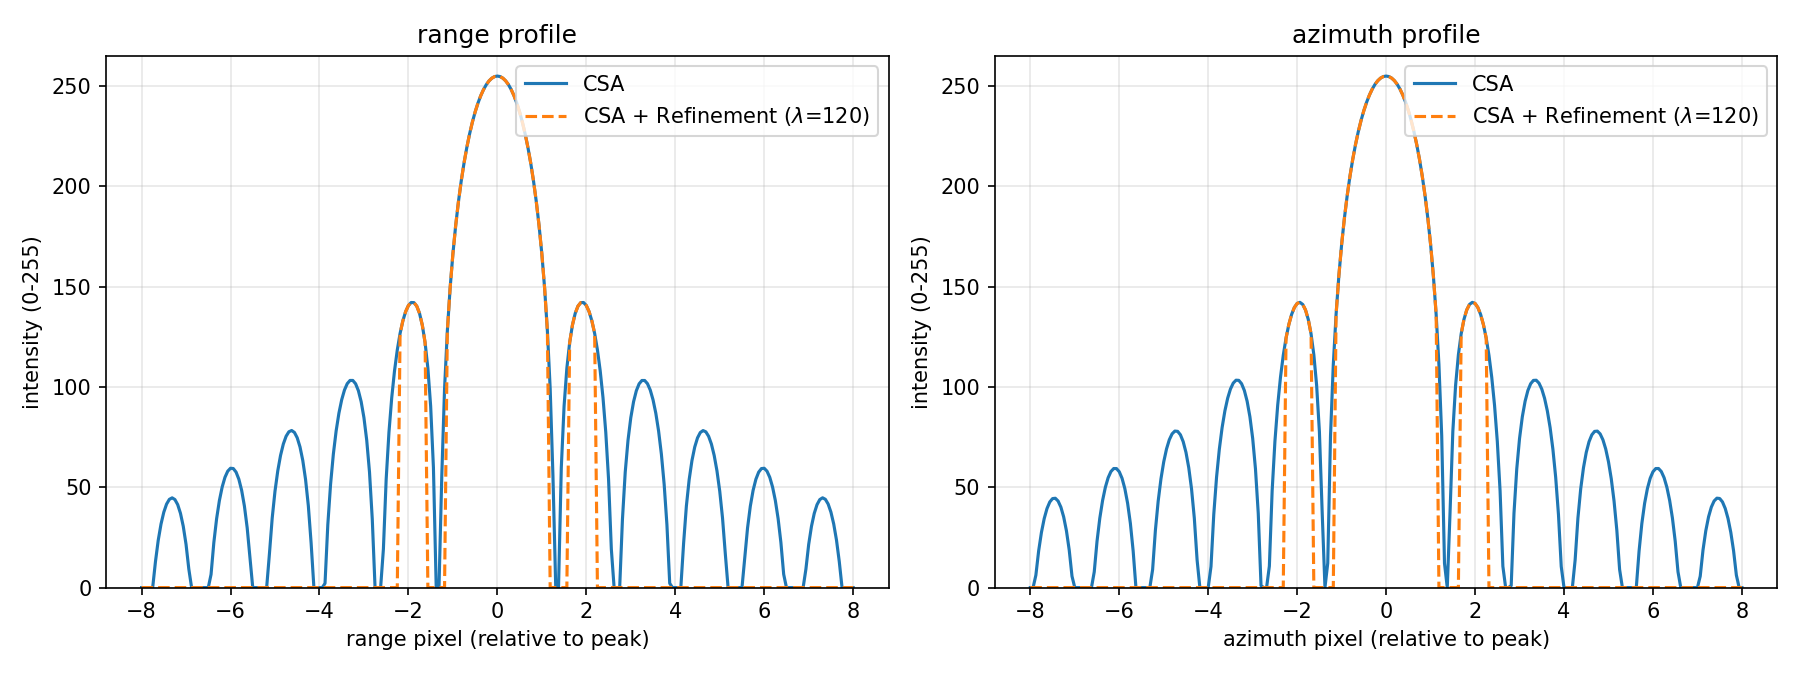
\includegraphics[width=\textwidth]{figures/single_point_threshold.png}
  \caption{Range (left) and azimuth (right) profiles of a single point target
    (0--255 intensity, 30~dB dynamic range) from CSA (solid) and CSA +
    refinement with $\lambda = 120$ (dashed). Pixels below $\lambda$ are set
    to zero, which is equivalent to Eq.~(7) with $\lambda$ added back.}
  \label{fig:single-point}
\end{figure}

% ── Comment 3 ─────────────────────────────────────────────────────────────────
\comment{Computational Complexity Analysis}{%
  Sections~1 and~2 state that CS can
  reduce the computational load, which supports real-time onboard
  processing. However, the one-step refinement is an additional step after
  CSA. Shouldn't the computational load therefore be higher than CSA alone?
  What baseline is the ``reduced computation'' measured against? What is the
  approximate computational load or execution time of the whole pipeline
  (CSA, refinement, and YOLO)?}

\response
The claim of low computational complexity in Sections~2.2 and~2.3 is made
relative to transformer-based methods, not to CSA alone. The requirement of
onboard processing is to achieve better performance than conventional CSA
without adding much computational complexity. A quantitative analysis of the
computational load of the whole pipeline (CSA, refinement, and YOLO) will be
conducted in future work.

% ── Comment 4 ─────────────────────────────────────────────────────────────────
\comment{Symbol Definitions and Dimensions}{%
  Fig.~3 uses $H$ to generate $Y$, while
  Eq.~(4) uses $S = [s_{m,n}]$ to denote the echo. What is the relationship
  between $Y$ and $S$? In addition, most symbols in the report are given
  without their dimensions or data types. For example, is $H$ a matrix? What
  is its dimension? Is it complex-valued, or real-valued intensity in the
  range 0--255? Do other symbols have the same issue?}

\response
The received echo is $\mathbf{Y} = \mathbf{S} + \mathbf{W}$, where
$\mathbf{S} = [s_{m,n}]$ in Eq.~(4) is the noise-free echo synthesized from the
scene $\mathbf{H}$, and $\mathbf{W}$ is the thermal noise, modeled as i.i.d.\
circular complex Gaussian. In the current experiments, $\mathbf{W}$ is set to
zero, i.e., $\mathbf{Y} = \mathbf{S}$. $\mathbf{H}$ is a complex-valued $M \times N$
matrix. For detection, the CSA complex image is cropped to $800 \times 800$ pixels and
converted to a real-valued 8-bit intensity image (30~dB dynamic range mapped
to 0--255), on which the threshold $\lambda = 120$ is applied. The main symbols
in the report, with their dimensions and data types, are listed in
Table~\ref{tab:symbols}; we will add this information to the report.

\begin{table}[H]
  \centering
  \small
  \caption{Main symbols in the report, with their dimensions and data types.}
  \label{tab:symbols}
  \begin{tabular}{lll}
    \toprule
    Symbol & Description & Type / dimension \\
    \midrule
    \multicolumn{3}{l}{\textit{Echo and image}} \\
    $M$, $N$ & Numbers of azimuth and range samples & Positive integers \\
    $m$, $n$ & Azimuth and range sample indices & Integers \\
    $\mathbf{Y}$ & Received echo & $\mathbb{C}^{M \times N}$ \\
    $\mathbf{S} = [s_{m,n}]$ & Noise-free echo, Eq.~(4) & $\mathbb{C}^{M \times N}$ \\
    $\mathbf{W}$ & Thermal noise & $\mathbb{C}^{M \times N}$ \\
    $\mathbf{H}$ & Scene reflectivity & $\mathbb{C}^{M \times N}$ \\
    $\mathbf{H}_{\mathrm{CSA}}$ & CSA complex image & $\mathbb{C}^{M \times N}$ \\
    $\hat{\mathbf{H}}$ & Refined complex image, Eq.~(6)--(7) & $\mathbb{C}^{M \times N}$ \\
    -- & Intensity image fed to YOLO & $\{0, \dots, 255\}^{800 \times 800}$ \\
    \midrule
    \multicolumn{3}{l}{\textit{Operators and regularization}} \\
    $\mathcal{A}(\cdot)$ & Forward operator, Eq.~(1) & $\mathbb{C}^{M \times N} \to \mathbb{C}^{M \times N}$ \\
    $R(\cdot)$ & Sparsity regularizer, Eq.~(1) & $\mathbb{C}^{M \times N} \to \mathbb{R}_{\ge 0}$ \\
    $\lambda$ (Eq.~(1), (6)--(7)) & Regularization parameter / threshold & Real scalar, $\ge 0$ \\
    $\mathcal{S}_\lambda(\cdot)$ & Soft-thresholding, Eq.~(7) & $\mathbb{C} \to \mathbb{C}$, element-wise \\
    \bottomrule
  \end{tabular}
\end{table}

% ── Appendix A ────────────────────────────────────────────────────────────────
\newpage
\section*{Appendix A: Unitarity of the CSA Matrix}

This appendix supports the response to Comment~1 by showing that the CSA
imaging operator, written as a matrix $\boldsymbol{\Phi}$, is unitary.

\subsection*{A.1 Vectorization}
The echo $\mathbf{Y}$ and the image $\mathbf{H}$ are both complex-valued
$M \times N$ matrices, where $M$ and $N$ are the numbers of azimuth and
range samples. The operator $\mathrm{vec}(\cdot)$ stacks the columns of a
matrix into one long column vector:
\begin{equation*}
  \mathbf{y} = \mathrm{vec}(\mathbf{Y})
    = \begin{bmatrix} \mathbf{Y}_{:,1} \\ \vdots \\ \mathbf{Y}_{:,N} \end{bmatrix}
    \in \mathbb{C}^{MN},
  \qquad
  \mathbf{h} = \mathrm{vec}(\mathbf{H}) \in \mathbb{C}^{MN},
\end{equation*}
where $\mathbf{Y}_{:,n}$ is the $n$-th column of $\mathbf{Y}$. Vectorization
only rearranges the entries, so it does not change the norm:
$\|\mathbf{Y}\|_F = \|\mathbf{y}\|_2$. It also turns every 2-D operation in
CSA into a matrix--vector product, which allows the whole algorithm to be
written as a single matrix.

\subsection*{A.2 CSA Flow in Matrix Form}
CSA consists of the following steps: azimuth FFT, chirp scaling, range FFT,
range compression and bulk RCMC, range IFFT, azimuth compression and residual
phase compensation, and azimuth IFFT. In matrix form,
\begin{equation*}
  \boldsymbol{\Phi} = \mathbf{F}_{a}^{-1}\mathbf{P}_{3}\,
                      \mathbf{F}_{r}^{-1}\mathbf{P}_{2}\,
                      \mathbf{F}_{r}\mathbf{P}_{1}\,\mathbf{F}_{a},
\end{equation*}
where
\begin{itemize}
  \item $\mathbf{F}_{a} = \mathbf{I}_{N} \otimes \mathbf{F}_{M}$ is the
        azimuth FFT (applied within each column) and $\mathbf{F}_{r} =
        \mathbf{F}_{N} \otimes \mathbf{I}_{M}$ is the range FFT (applied
        within each row). Here $\otimes$ is the Kronecker product and
        $\mathbf{F}_{K}$ is the $K$-point DFT matrix.
  \item $\mathbf{P}_{1}$ is the chirp scaling, $\mathbf{P}_{2}$ is the range
        compression and bulk RCMC, and $\mathbf{P}_{3}$ is the azimuth
        compression and residual phase compensation.
\end{itemize}
Since a product of unitary matrices is unitary, it suffices to show that each
factor is unitary.

\subsection*{A.3 Chirp Scaling and Phase Compensation}
Chirp scaling and phase compensation are both Hadamard (element-wise)
products of the data with a complex exponential array. For chirp scaling in
the range-Doppler domain,
\begin{equation*}
  \mathbf{X}_{\mathrm{out}} = \mathbf{E}_{1} \odot \mathbf{X}_{\mathrm{in}},
  \qquad [\mathbf{E}_{1}]_{m,n} = e^{j\phi_{1}(f_{a,m},\,\tau_{n})},
\end{equation*}
where $\phi_{1}$ is real. After vectorization, the Hadamard product becomes
multiplication by a diagonal complex exponential matrix:
\begin{equation*}
  \mathrm{vec}(\mathbf{X}_{\mathrm{out}})
    = \mathbf{P}_{1}\,\mathrm{vec}(\mathbf{X}_{\mathrm{in}}),
  \qquad
  \mathbf{P}_{1} = \mathrm{diag}\!\left(\mathrm{vec}(\mathbf{E}_{1})\right)
    = \mathrm{diag}\!\left(e^{j\phi_{1,1}}, \dots, e^{j\phi_{1,MN}}\right),
\end{equation*}
with $MN$ diagonal entries. Since every diagonal entry has unit magnitude,
\begin{equation*}
  \mathbf{P}_{1}^{H}\mathbf{P}_{1}
    = \mathrm{diag}\!\left(|e^{j\phi_{1,1}}|^{2}, \dots,
                           |e^{j\phi_{1,MN}}|^{2}\right)
    = \mathbf{I},
\end{equation*}
so $\mathbf{P}_{1}$ is unitary. The same holds for $\mathbf{P}_{2}$ and
$\mathbf{P}_{3}$, which differ from $\mathbf{P}_{1}$ only in the phase
function.

\subsection*{A.4 DFT}
The normalized DFT matrix $\mathbf{F}_{K}$ is unitary, and the Kronecker
product of unitary matrices is unitary, so $\mathbf{F}_{a}$ and
$\mathbf{F}_{r}$ are unitary. Our implementation uses an unnormalized
forward FFT (a factor of $\sqrt{K}$) and an inverse FFT divided by $K$ (a
factor of $1/\sqrt{K}$). Since each axis has exactly one FFT and one inverse
FFT, the two factors cancel.

\subsection*{A.5 Conclusion}
All factors of $\boldsymbol{\Phi}$ are unitary, so $\boldsymbol{\Phi}$ is
unitary: $\boldsymbol{\Phi}^{H}\boldsymbol{\Phi} = \mathbf{I}$ and
$\boldsymbol{\Phi}^{-1} = \boldsymbol{\Phi}^{H}$.

\end{document}
